\documentclass[12pt,a4paper,oneside]{report}

\usepackage{titlesec}
\usepackage{geometry}
\usepackage{graphicx}
\usepackage{booktabs, chemformula}
\usepackage{titlesec, blindtext, color}
\newcommand\tab[1][1cm]{\hspace*{#1}}

 \geometry{
 a4paper,
 top=35mm,
bottom=30mm,
bindingoffset=0.0in
 }
\pagenumbering{arabic} 

\pagestyle{headings}

\newcommand{\dspaceon}{\renewcommand{\baselinestretch}{1.3}\large\normalsize}
\newcommand{\dspaceoff}{\renewcommand{\baselinestretch}{1}\large\normalsize}

\graphicspath{ {images/} }

\definecolor{gray75}{gray}{0.75}
\newcommand{\hsp}{\hspace{20pt}}
\titleformat{\chapter}[hang]{\Large\bfseries}{\thechapter\hsp\textcolor{gray75}{$|$}\hsp}{0pt}{\Large\bfseries}
\titleformat{\section}{\normalfont\large\bfseries}{\thesection}{1em}{}


\begin{document}
\begin{titlepage}
%\newgeometry{left=20mm,right=20mm,top=2.5cm,bottom=2cm}


\thispagestyle{empty}
\setlength\headheight{0pt} 
\begin{center}


\hfill 
\includegraphics[width=0.45\linewidth]{oxlogo.jpg}            


        \vspace{3cm}
        {\LARGE Computer Science and Engineering Department\\
"Politehnica" University of Timisoara \par}
        \vspace{3cm}

        {\Large\bfseries An analysis of the relationship between structural and logical\\ dependencies in software systems \par}
        
        \vspace{3cm}
        {\Large\itshape Adelina Diana Stana\par}
        \vspace{0.25cm}

\vspace{1cm}
Coordinated by\par
Assoc Prof.~Ioana \textsc{Sora}\par
\vspace{1.5cm}
\large
\today

\end{center}

\clearpage
\restoregeometry
\end{titlepage}


\tableofcontents

\newpage

\chapter{Introduction}

\section {State of the art}
\tab Software systems are continuously in change. As long as the software system is used the changing process is never finished. Changes can be triggered by new features , defects, new technologies, system refactoring for maintainability.\\ Software maintenance can be made during the development process by maintaining the already implemented features, while developing new ones or at the endofthedevelopmentprocesswhenthesystemisno longer open to new features requested by the client and the maintenance is only made for the existing ones. From an architectural point of view,a system is stable when a change in one component of the system does not affect the other components .This rule applies recursively also inside the components.\\ 
\tab The ideal situation presumes that changes in one part can be made without changing parts that are in a dependency relation with that part. Those dependencies affect the maintainability of the system and increase the realization effort of any problem that appears during the maintenance time. Studying only the structural dependencies of the system is not enough to get a clear overview of the system dependencies. For more precise results is needed a study that combines structural dependencies and logical dependencies. \\ We have analysed 19 open-source software systems of different sizes to investigate the links between structural dependencies and logical dependencies. 


\tab During the development process of a software system new classes and new methods to the existing classes are added in order to fulfill new functionalities. All of the adding actions from above have a direct impact on the system structural dependencies. Those are the result of the source code analysis of the system. \\The source code is any static, textual, human readable, fully executable description of a computer program that can be compiled automatically into an executable form \cite{ct1}.\\On the other hand logical dependencies also can be added during the development process. Logical dependencies refer to those depencencies between entities that are not always visible through source code analysis (Figure \ref{fig:fig1}).

\begin{figure}[h]
\centering
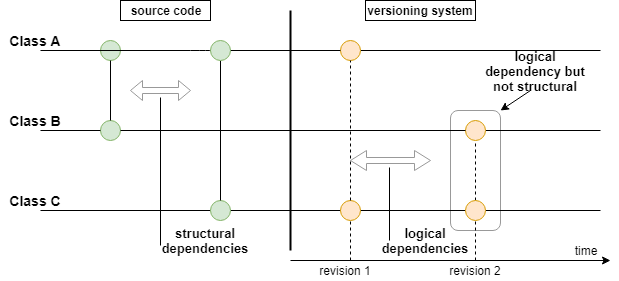
\includegraphics[scale=0.60]{fig1.png}
\caption{Relationships between structural and logical dependencies }
\label{fig:fig1}
\centering
\end{figure}

Logical dependencies can be easily extracted from the versioning system (e.g. Subversion , Git) revisions. 


\section{Purpose of the project}
In this paper we intend to understand better the intersection between structural dependencies and logical dependencies and their impact over the system (Figure \ref{fig:fig2}). 
To be done ...


\begin{figure}[h]
\centering
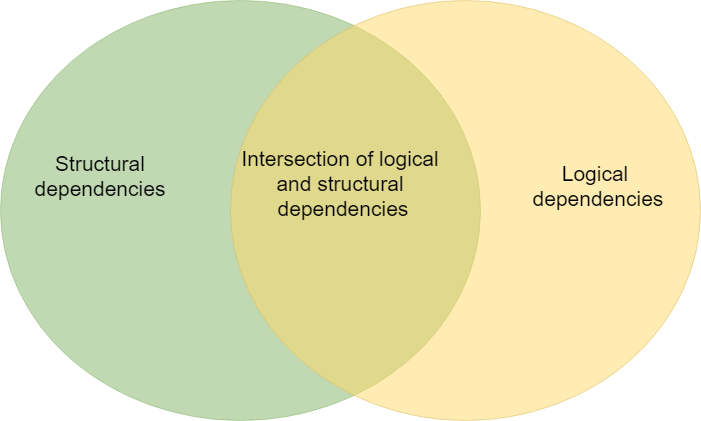
\includegraphics[scale=0.4]{fig2.png}
\caption{Venn Diagram showing the intersection between structural and logical dependencies }
\label{fig:fig2}
\end{figure}

\chapter{Theoretical aspects}

\section {State of the art}

\tab During the development process of a software system new classes and new methods to the existing classes are added in order to fulfill new functionalities. All of the adding actions from above have a direct impact on the system structural dependencies. Those are the result of the source code analysis of the system. \\The source code is any static, textual, human readable, fully executable description of a computer program that can be compiled automatically into an executable form \cite{ct1}.\\On the other hand logical dependencies also can be added during the development process. Logical dependencies refer to those depencencies between entities that are not always visible through source code analysis. Logical dependencies can be easily extracted from the versioning system (e.g. Subversion , Git) commits.  (Figure \ref{fig:fig1}).

\tab The ideal situation presumes that changes in one part can be made without changing parts that are in a dependency relation with that part. Those dependencies affect the maintainability of the system and increase the realization effort of any problem that appears during the maintenance time. Studying only the structural dependencies of the system is not enough to get a clear overview of the system dependencies. For more precise results is needed a study that combines structural dependencies and logical dependencies. \\ We have analysed 19 open-source software systems of different sizes to investigate the links between structural dependencies and logical dependencies. 


\begin{figure}[h]
\centering
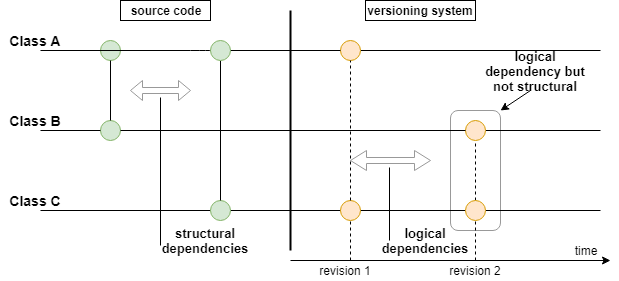
\includegraphics[scale=0.60]{fig1.png}
\caption{Relationships between structural and logical dependencies }
\label{fig:fig1}
\centering
\end{figure}

\section{Software dependencies}
\tab A dependency is created by two elements that are in a relationship and indicates that an element of the relationship, in some manner, depends on the other element of the relationship. In this case, if one of these elements change, there could be an impact to the other \cite{ct2}. Dependencies are discovered by analysis of source code or from an intermediate representation such as abstract syntax trees \cite{ct3} .

\section{Structural dependencies}
\tab Structural dependencies (a.k.a syntactic dependencies or structural coupling) are the result of source code analysis. Each source code file can contain one or more classes \cite{ct4}.\\

In object-oriented programming, a class is an template for creating objects that provides initial values for member variables and implementations of functions or methods. \cite{oopconcept}\\
\tab In the following we will present the class components and how those components can introduce software dependencies with other classes.

Class components to discuss :
\begin{itemize}
  \item Class name. Inheritance.
  \item Comments.
  \item Attributes. 
   \item Constructors.
   \item Methods.
\end{itemize}


\subsubsection{Class name. Inheritance}
The user-defined objects are created using the class keyword. The class is a blueprint that defines a nature of a future object. 
The name of the class is the name located after the keyword class. During the structural analysis of the projects the classes names are extracted in order to identify the structural dependencies elements names .

\begin{lstlisting}[language=java, caption={Class declaration.}]
public class A {
}
public class B extends A {
}
\end{lstlisting}

A structural dependency between a class and other class can be given by inheritance. Inheritance can be defined as the process where one class acquires the properties of another class \cite{oopconcept} .\\
The class which inherits the properties of other class is known as subclass and the class whose properties are inherited is known as superclass (a.k.a base class, parent class). The name of the superclass is the name located after the keyword extends .

\subsubsection{Comments}
Comments are statements that are not executed by the compiler and interpreter. The comments can be used to provide information about a variable, method or any other statement. There are multiple types of comments :\\

\textit{/* text */} -  ignores characters from begining of /* to */.\\
\textit{/** documentation */} -  indicates a documentation comment, just like comments that use /* and */.\\
\textit{// text} -  ignores everything from // to the end of the line.\\ 

Comments never introduce any kind of structural dependencies. They are used just for the source code intelligibility.

\subsubsection{Attributes}

Attributes represent the state of the object because they store the information about the object. An attribute is another term for a field. \\

\textit{private B b;}\\
The keyword private signifies that a method or variable can be accessed only within the declaring object. The keyword public allows access also from outside of the object \cite{oop2}, \cite{ct11} .

The attributes or members of a class can lead to structural dependencies between the class and the class types of the attributes.

\subsubsection{Constructors}

A constructor of a class is a member function that is executed whenever we create a new object of that class.  A parameterized constructor introduces new structural dependencies by its parameters.

\subsubsection{Methods}

Some of these attributes and methods are publicly visible from outside the object:  the interface. Other
attributes and methods are for private use of the object itself : the implementation. Either ways when studying structural dependencies the publicity of an attribute or of a method is irrelevant. \cite{oopconcept} The relevant part is the type of the attribute or the return type and the parameters of the method. A method can introduce structural dependencies in three ways : by its return type , by its call parameters or by its local variables .\\

\tab On the other hand, even though in some of the cases if class A depends on class B , changes in class B can produce changes in class A, but not the other way around \cite{ct5} . There are other cases in which if class A depends on class B, changes in class B can produce changes in class A and viceversa if we are speaking in the context of a new feature implementation that implies changing return types and adding new methods. So we will consider structural dependencies as bidirectional relationships, "classA depends on class B" and "class B depends on class A".\\ \tab The choice of building bidirectional relationships is motivated by the fact that we cannot establish for the moment the direction of the logical dependencies of the system. So in order to have a omogeninty between the logical and structural dependencies analysis results, we will take both of the relationships types as bidirectional. 

\section{Logical dependencies}
\subsection{Version control systems}
In computer software engineering, revision control is any kind of practice that tracks and provides control over changes to source code. Software developers sometimes use revision control software to maintain documentation and source code.\\
At a basic level, developers could retain multiple copies of the different versions of the program and label them appropriately. This method can work but it is inefficient as many copies of the program have to be maintained. Because of this, systems to automate some or all of the revision control process have been developed. 
\\ 
\tab Among the keywords used in a versioning system we can mention:\\
\textit{\textbf{Repository}} -  is a virtual storage of a project. It allows to save versions of the code, which can be access when needed.\\
\textit{\textbf{Master/Trunk}} - the main body of development, originating from the start of the project until the present.\\
\textit{\textbf{Branch} }- a copy of code derived from a certain point in the master that is used for applying major changes to the code while preserving the integrity of the code in the master. The changes are usually merged back into the master.\\
\textit{\textbf{Revision}} - changes are usually identified by a number or letter code, that code is known as "revision".\\


\subsection{Definition}

\tab  In software engineering, we use co-evolution to represent the phenomenon in software evolution that change in one component C2 in response to a change in another component C1 \cite{ct5}, \cite{ct6}, \cite{ct8}. 
There are differences between co-evolution and evolutionary coupling.\\
\tab Co-evolution is the result of cause–effect changes between two components: changes to one component require changes to another component. On the other hand, evolutionary coupling is based on the evolution history of two components and is a measurement of the observation that two components are changed at the same time.\\ 
\tab  Modifications made to two components at the same commit do not necessarily indicate the co-evolution of the two. These modifications could be completely unrelated.\\ So, evolutionary coupling could also be determend accidentally by two components changing in the same commit and it will bring noise to the measurement of evolutionary coupling.  \cite{ct5} \\ We will try to filter that noise by setting different thresholds in the process of analysing the systems.

\tab The versioning system contains the long-term change history of every file. Each project change made by an individual at certain point of time is contained into a commit \cite{ct7}.All the commits are stored in the versioning system cronologicaly and each commit has a parent. The parent commit is the baseline from which development began, the only exeption to this rule is the first commit which has no parent. We will take into consideration only \textit{commits that have a parent} since the first commit can include source code files that are already in development (migration from one versioning system to another) and this can introduce reduntant logical links \cite{ct8} .\\

\tab The number of files changed in a commit can influence the logical dependencies. A relatively big number of files changed can indicate a merge of all changes from another branch as a single commit or a folder renaming. This can lead to a number of logical dependencies that are redundant since the files are not actualy changing in the same time.The logical dependencies are splitted into three categories :\\ \\
\textit{\textbf{Category 1:} Dependencies found in commits with less than 5 source code files changed.}\\
\textit{\textbf{Category 2:} Dependencies found in commits with more than 5 files changed but less than 20. }\\
\textit{\textbf{Category 3:} Dependencies found in commits with more than 20 files.}\\

\tab Also, files that changed only by comments change can lead to redundant logical dependencies. If class A and class B change together but the only change was a change in the comments then there may not be any logical dependency between them. 
For each category mentioned above, two dependencies analysis will be made:
\textit{\textbf{A:} Considering comments  as valid changes.}
\textit{\textbf{B:} Considering comments  as redundant changes. }
In the second case if class A and class B change together but the only change found is a comment change then between class A and B will not be set a logical dependency.\\

\tab Another filtering method that can lead to a more accurate results is to count the occurrences of the logical dependencies. If class A and class B change together but only once during all the commits from the active branch the class A and B may or may not represent a logical dependency.


\chapter{Tool usage}
The tool has multiple usage options that will be presented in the following sections. 
\section{Loading a project}
\begin{figure*}[h]
\centering
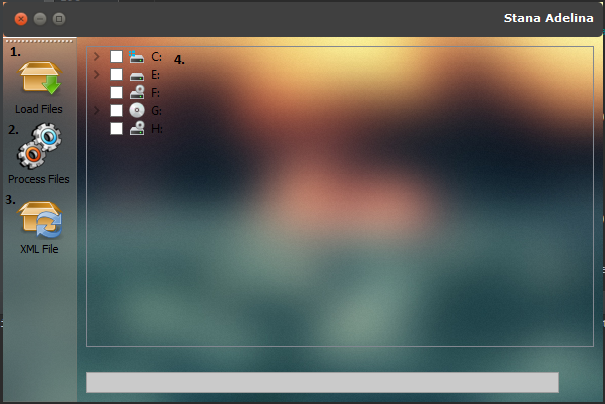
\includegraphics[width=\textwidth]{tool.png}
\caption{User interface}
\label{fig:figtool}
\end{figure*}

\tab For building the logical and structural dependencies the project root folder is needed. The tool offers a tree view of all the file system as shown in 4. of figure \ref{fig:figtool} . \\ The user does not have to select manualy each file, the selection of a folder implies the automatic selection of all subfolders and files. Also there is no need to select only the source code files, the tool processes all the files selected and only the ones with the accepted extensions are taken into consideration. To load all the files selected in the tool the button \textit{Load Files} needs to be pressed shown in 1. of figure \ref{fig:figtool} .

\section{Processing files}
\tab The next and final step to obtain the results is to press \textit{Process Files} button shown in 2. in figure \ref{fig:figtool} . The tool has a process bar wich shows to the user the percent of files processed as shown in figure \ref{fig:figloading} .

\begin{figure*}[h]
\centering
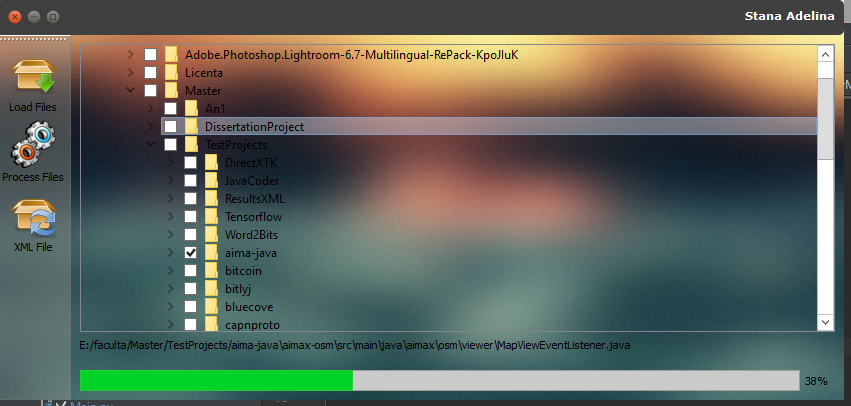
\includegraphics[width=\textwidth]{loading.png}
\caption{Loading files process bar}
\label{fig:figloading}
\end{figure*}

 This step implies the creation of XML files corresponding to the source code files , identifying the Git repository of the project, optaining all the structural and logical dependencies and their overlapings graphs .

\section{Load XML of previous run}
\tab Once the logical and structural dependencies are extracted the tool builds and saves a XML file with all the informations collected. So, if a project needs to be reanalysed, only the XML file needs to be uploaded. In this way a lot of time is saved since is no need to recolect data from source code files and commits. To perform this action the Load XML button (number 3. in figure \ref{fig:figtool} ) needs to be pressed and a file browse dialog will appear so the user can choose the file as shown in figure \ref{fig:figxmlload}.
\begin{figure*}[h]
\centering
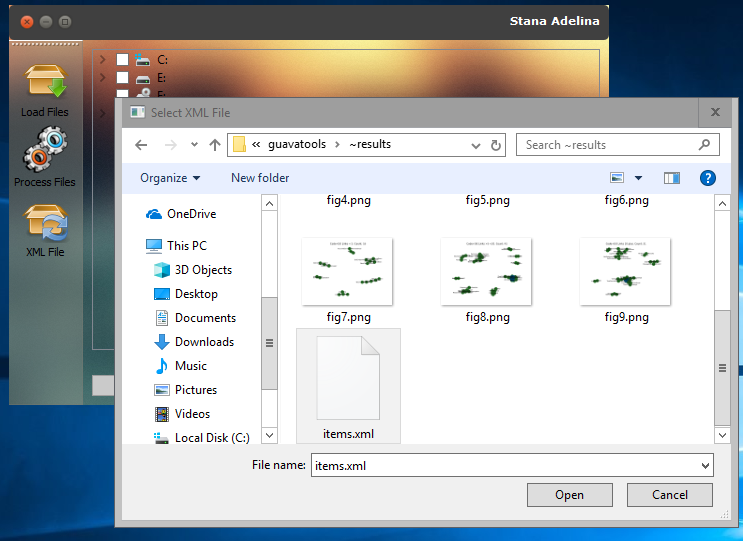
\includegraphics[width=\textwidth]{xmlload.png}
\caption{Loading a XML of a previous run.}
\label{fig:figxmlload}
\end{figure*}
\\
\tab The xml file is saved in the \textit{~results} folder created by the tool. The tool creates for each project analysed 3 folders , 2 temporary folders which are deleted after the process run and one results folder which is not deleted after the process run. The first temporary folder is the one that contains all the source code coresponing XML files , the second contains all the differences files extracted from the project commits. The last one is the \textit{~results} folder which contains all the graphics generated and the XML file with all the data extracted.
\\
\\
\\
\section{Output graphics}
 
\tab The output of the analysis made by the tool is represented as a series of graphics. Each graphic has in it's title the semnification of the displayed values and their counter (Figure \ref{fig:gitlinks}). For example for structural and logical dependencies found in files with less then 5 files changed the tool will display a graphic with the name "Overlapping structural and logical for more the 5 files changed . Counter : numberOfOverlaps" .
The tool will create graphics for the following casess: 
\begin{itemize}
  \item Structural dependencies found.
  \item Logical dependencies found in commits with less then 5 files changed.
  \item Logical dependencies found in commits with more then 5 files changed and less the 20.
  \item Logical dependencies found in commits with more then 20 files changed.
  \item The intersection of all the logical dependencies from all the 3 categories.
  \item The intersection between structural and logical dependencies found in commits with less then 5 files changed.
  \item The intersection between structural and logical dependencies found in commits with more then 5 files changed and less the 20.
  \item The intersection between structural and logical dependencies found in commits with more then 20 files changed .
  \item The intersection between structural dependencies and the intersection of all the logical dependencies from all the 3 categories .
\end{itemize}

Figure \ref{fig:gitlinks}
\begin{figure*}[h]
\centering
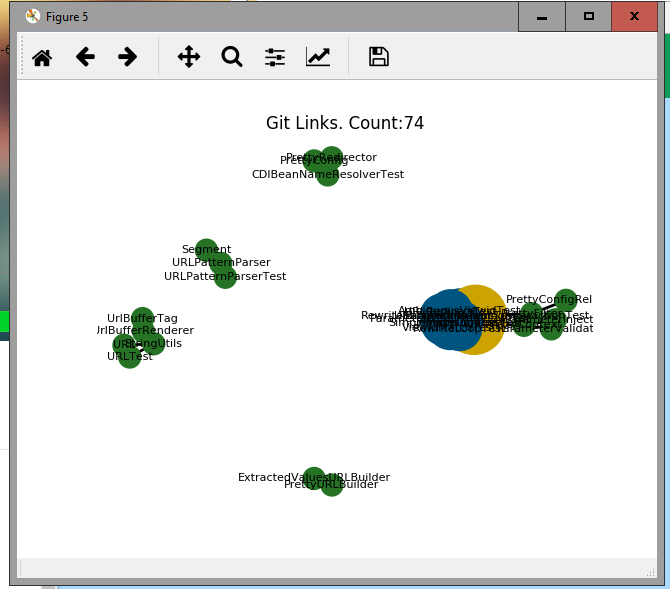
\includegraphics[width=\textwidth]{gitlinks.png}
\caption{Output graph from the analysis}
\label{fig:gitlinks}
\end{figure*}


\chapter{Implementation details}
The programming language used for developing the tool is \textit{\textbf{Python}} . Python is a general-purpose interpreted, object-oriented, and high-level programming language. It was created by Guido van Rossum during 1985- 1990. \cite{python}
In addition \textit{\textbf{PyQt}} is used as UI layer. PyQt is a Python binding for the Qt cross-platform C++ framework. 

\section{Processing phases}
\tab In order to build structural and logical dependencies the tool that takes as input the source code repository and builds the required software dependencies . The workflow can be delimited by three major steps as it follows  (Figure \ref{fig:fig3}):  \\\\
\textit{\textbf{Step 1:} Extracting structural dependencies.}\\
\textit{\textbf{Step 2:} Extracting logical dependencies.}\\
\textit{\textbf{Step 3:} Processing the information extracted and graphics generation.}

\begin{figure}[h]
\centering
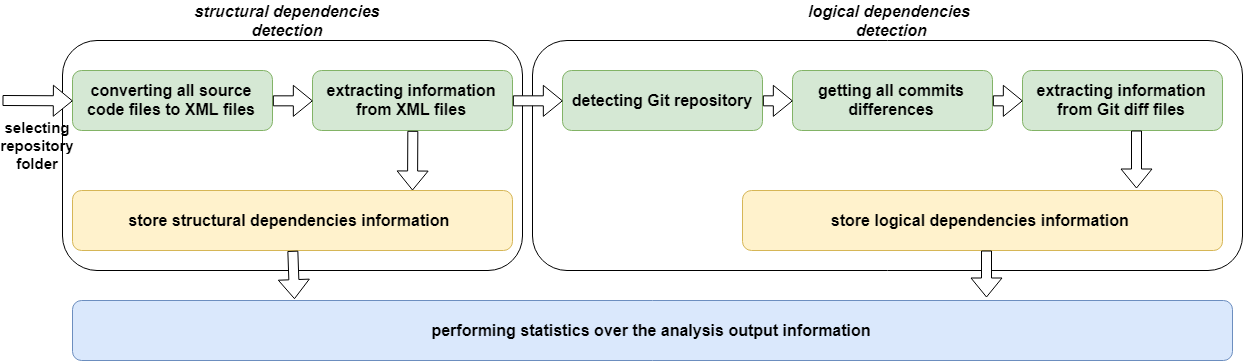
\includegraphics[width=\textwidth]{fig3.png}
\caption{Processing phases}
\label{fig:fig3}
\end{figure}


\section{Architecture}

\begin{figure}[h]
\centering
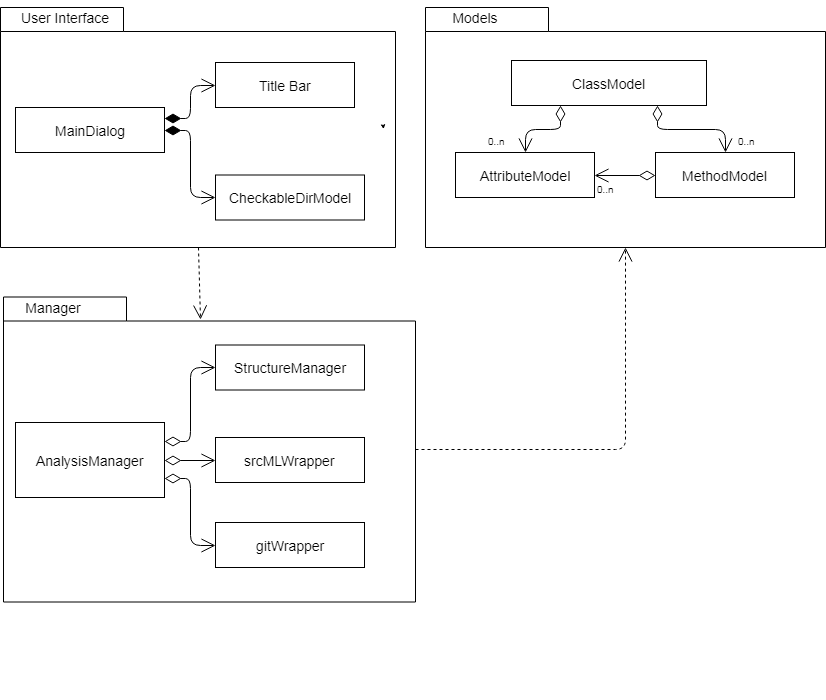
\includegraphics[width=\textwidth]{classdiagram.png}
\caption{UML diagram of the tool}
\label{fig:figdiagram}
\end{figure}

 \textit{\textbf{MainDialog}} is responsible for the User Interface creation . This class also handles the events from the user (process button pressed , load files button pressed, close window button pressed). MainDialog uses the TitleBar class for the title bar creation and CheckableDirModel for file system tree view. \\

The \textit{\textbf{ CheckableDirModel}} inherits QDirModel class which provides a data model for the local filesystem.In addition CheckableDirModel adds checkboxes to each filesystem item for a more easyer selection and returns a list of all files selected. \\

\textit{\textbf{ TitleBar}} inherits QMenuBar class which provides a horizontal menu bar. TitleBar class is used to create a new title bar, different from the one provided by Windows system . The class handles events like minimize , maximize and close window which are then emited to MainDialog class .\\

 A \textit{\textbf{ClassModel}} object contains all the informations extracted from the structural analysis about a class. ClassModel class contains a member for the name of the class , one for the parent name of the class and one for the xml file path in which the class was found. It also contains a list of MethodModels, a list of AttributeModels and 3 lists for git links, one for links found in commits with below 5 files changed , one for above 5 files changed and below 20 and one for links found in commits with above 20 files changed.The git links lists are lists of string objects. The class provides setters and getters for all the members mentioned above for retrieving and updating their values. \\

A \textit{\textbf{MethodModel}} object contains all the information extracted from the structural analysis about a method of a class. MethodModel contains a member for the name of the method and two lists of AttributeModels . One is used for the call parameters of the method and one is used for the local variables found inside the method.\\

 \textit{\textbf{AttributeModel}} contains two members , type and name. "Type" is used to identify the object type and "Name" is used to identify the object name. The class provides setters and getters for the members mentioned above for retrieving and updating their values. \\

 \textit{\textbf{AnalysisManager}} is created and called by  \textit{MainDialog}. MainDialog creates a AnalysisManager object and passes to it a list of source code files paths to be analysed and the parent folder path. The path to the parent folder is used to identify the Git repository. AnalysisManager is called each time the user triggers events in the User Interface. AnalysisManager calls the srcMLWrapper for XML conversion and XML files parsing and data extraction.\\ All the data extracted are passed to StructureManager. It also calls GitWrapper which interogates the project repository and saves all the commit differences in a temporary folder. The class is also responsable for parsing all the diff files and extracting the git links. The git links are passed to StructureManager which splits them into categories and setts them to the coresponding ClassModel object (figure \ref{fig:seq}). Finally is responsable for plotting the results of different queries (Example : all the overlappings between structural dependencies and logical dependencies extracted from commits with less then 5 files changed ) .\\

 \textit{\textbf{StructureManager}} contains all the ClassModels extracted  and is used by the AnalysisManager to save all datas extracted to an XML file and to load the datas extracted from an XML file (each project has an coresponding XML file that is created automaticaly after the analysis is done). Also is responsable to add the git links to the coresponding classes .\\

\textit{\textbf{srcMLWrapper}} has methods for converting source code files into XML files and to parse the resulting XML files in order to extract informations about classes , methods , members.\\

\textit{\textbf{GitWrapper}} identifies the git repository of the path given as a parameter and creates a temporary folder in which all the differences files are stored.


\begin{figure}
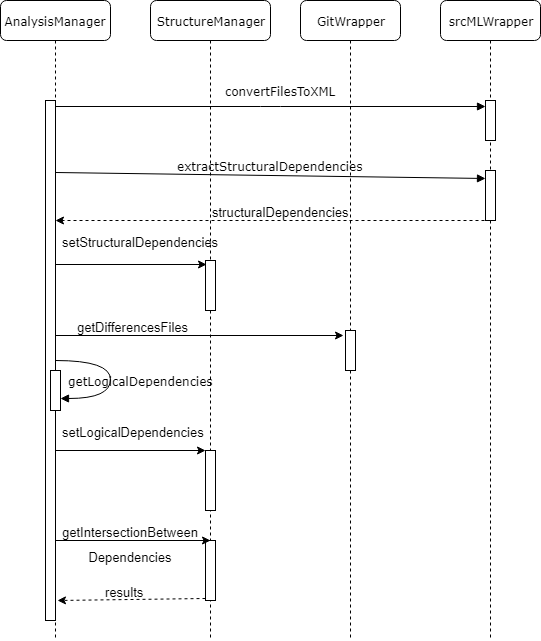
\includegraphics[scale=0.7]{flowdiag.png}
\caption{Sequence diagram}
\label{fig:seq}
\end{figure}

\section{User Interface}

\subsubsection{Creating MainDialog components}

MainDialog class inherits QMainWindow from PyQt which provides a main application window. The window is set as frameless window since a custom TitleBar will be attached to it. 

\begin{lstlisting}[language=python, caption={Create the title bar for the main window.}]
self.setWindowFlags(QtCore.Qt.FramelessWindowHint)
self.titleBar = TitleBar(self)
self.setMenuBar(self.titleBar)
\end{lstlisting}

In addition other widgets will be created : progress line , progress bar , tree view of the file system . All the above will be added after creation to the main layout of the window. There are two types of layouts in PyQt : \textit{QVBoxLayout} and \textit{QHBoxLayout} . The first layout lines up widgets vertically and the second horizontally.

\begin{lstlisting}[language=python, caption={Add widgets to the main window layout.}]
self.boxLayout = QVBoxLayout(self)

self.boxLayout.addWidget(self.tree)
self.boxLayout.addWidget(self.progressLine)
self.boxLayout.addWidget(self.progressBar)
\end{lstlisting}

\subsubsection{Creating Menus}
Qt implements menus in QMenu and QMainWindow keeps them in a QMenuBar. QAction is an abstraction for actions performed with a menubar and can be created with an icon and a name. After the creation, the action is connected to a method, so when we select a particular action, a triggered signal is emitted and the specified method executes. 

\begin{lstlisting}[language=python, caption={A menu creation with two actions.}]
processAction = QAction(QIcon('resources/run.png'), 'Process Files', self)
xmlLoadAction = QAction(QIcon('resources/load.png'), 'XML File', self)

processAction.triggered.connect(self.processFilesClicked)
xmlLoadAction.triggered.connect(self.loadXmlClicked)

self.toolbar.addAction(processAction)
self.toolbar.addAction(xmlLoadAction)
\end{lstlisting}

\section{Extracting software dependencies}
\subsection{srcML}
SrcML is an open source tool that converts in an XML format C/C\#/Cpp/Java source code. \cite{srcml1}\\
All the original source code files are kept and the corresponding XML files are created. Each source code file is converted in a single XML document.\\
 The srcML toolkit includes \textbf{source-to-srcML} and \textbf{srcML-to-source} translators:
\begin{itemize}
  \item source-to-srcML : is responsable for source code to XML conversion.
  \item srcML-to-source : is responsable for XML to source code conversion, so that the original source code document can be recreated from the srcML XML file.
\end{itemize}

The srcML XML contains of all text from the source code file and XML tags. The file contains all the syntactic structures from the code (e.g., classes, structures, functions, function call, destructors, methods, if statements, for statements, switch statements, etc.).\cite{srcml2}
An example of the XML representation can be found in Figure \ref{fig:figxml} .

\begin{figure*}[h]
\centering
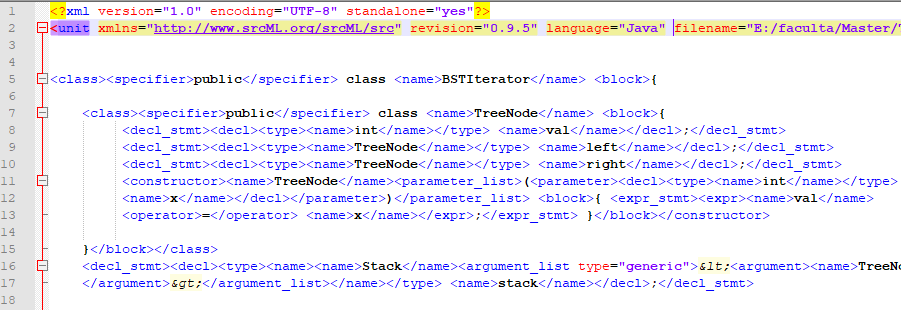
\includegraphics[width=\textwidth]{xmlscreenshot.PNG}
\caption{Example of XML representation of source code.}
\label{fig:figxml}
\end{figure*}

\subsection{Convert files to XML using srcML}
\tab As mentioned above, for conversion from source code to XML we will use srcML.
Through UI the user can choose the main folder of the to-be analysed project. The tool will walk trough all the subfolders and files of the folder and will get only the files that are source code files (files with extension such as .cpp ,.c++, .h , .java).
\begin{lstlisting}[language=python, caption={Walk through the given directory and extract only source code files}]
for path, dirs, files in os.walk(self.filePath(index)):
    for filename in files:
        if QtCore.QFileInfo(filename).completeSuffix() in acceptedSuffix:
             selection.add(os.path.join(path, filename))
\end{lstlisting}

The next step is to convert each file to XML. The conversion will be made through calls to srcML using the \textbf{subprocess} module . The subprocess module allows to spawn new processes, connect to their input/output/error pipes, and obtain their return codes. 
Arguments to pass to srcML :
\begin{itemize}
  \item the path to the file to-be-converted
  \item "-o" option , stands for outputting to a file 
  \item the output file path
\end{itemize}

\begin{lstlisting}[language=python, caption={Convert source code to XML using subprocess module.}]
def convertFiles(self, file):
    file_name = os.path.basename(file)
    file_xml = self.workingDir + "/"+file_name + ".xml"
     cmd = "srcml \""+file+"\" -o \""+file_xml+"\""
     rez = subprocess.Popen(cmd, shell=True, stdout=subprocess.PIPE).stdout.read()
\end{lstlisting}

\subsection{Extracting structural dependencies from XML}
\subsubsection{The ElementTree library}
For XML parsing we used \textbf{The ElementTree} library.It includes tools for parsing XML using event-based and document-based APIs, searching parsed documents with XPath expressions, and creating or modifying existing documents.
Parsing an entire document with parse() returns an ElementTree instance. The tree knows about all of the data in the input document, and the nodes of the tree can be searched or manipulated.

\begin{lstlisting}[language=python, caption={Import and create ElementTree instance}]
 import xml.etree.ElementTree as ET
 tree = ET.parse(file)
\end{lstlisting}

\subsubsection{Class extraction}
\textbf{Element.findall("name")} finds only elements with the tag "name" which are direct children of the current element. The items returned by findall() are Element objects, each representing a node in the XML tree. Each Element has attributes for accessing the data of the XML.
\begin{lstlisting}[language=python, caption={Get name of  Element item. }]
 def getName(self, item):
        if item is not None:
            text = item.text
            if text is None:
                return self.getText(item.find("name"))
            return text
\end{lstlisting}

\tab One xml file can contain one or more class types. Also one class can contain other class definitions so the parsing will be made recursively. Each time a new class is found a ClassModel object is created  and added to a list. 


\begin{lstlisting}[language=python, caption={Recursively find all the classes from XML file.}]
def getClassModelJava(self, file, root):
        classList = []

        for item in root.findall("{http://www.srcML.org/srcML/src}class"):
            className = self.getName(item)
            insideClassList = self.getClassModelJava(file, item)

            if insideClassList:
                classList.extend(insideClassList)

            classModel = ClassModel()
            classModel.setFile(file)
            classModel.setName(className)
		....
\end{lstlisting}

\subsubsection{Method extraction}
A ClassModel has a list of attributes and a list of methods. The methods are relevant because their call parameters and attributes can create structural dependencies. In order to get the parameters names we will look for \textbf{parameter\_list} tag inside the tree. For attributes we will look for \textbf{decl\_stmt} tag .
\begin{lstlisting}[language=python, caption={Get the parameter list of a method.}]
method = MethodModel()
method.setType(element_type)
method.setName(element_name)

for param in self.getAttributes(self.getItem(decl, "parameter_list"), "parameter"):
	method.addArgs(param)
....
classModel.addMethod(method)
\end{lstlisting}

\subsubsection{Attribute extraction}
Both ClassModel and MethodModel have a list of attributes.  Those attributes give the structural dependencies of the class . The call parameters of a function are also considered as attributes . We will refer to the AttributeModel class as a class that contain the information required to identify one side of the structural depencency link. The other side is the ClassModel containing the AttributeModel . 
\begin{lstlisting}[language=python, caption={Get the attributes list of a method or class.}]
for a in self.getAllItems(decl, "decl"):
   element_type = self.getType(a)
   element_name = self.getName(a)

   attribute = AttributeModel()
   attribute.setType(element_type)
   attribute.setName(element_name)

   attributes.append(attribute)
 return attributes
\end{lstlisting}

\section{Extracting logical dependencies}

\tab The second step of the analysis is to extract logical dependencies from the versioning system.  Changes can be made by many individuals over the years.\\ 
Changes include the creation and deletion of files as well as edits to their contents. Each change (this can include changes in multiple files) made by an individual at certain point of time is contained into a commit\cite{ct7}. \\ The tool looks through the repository and gets all the existing commits, for each commit a differences file will be made .After all the differences files are stored , all the files are parsed and logical dependencies are build. 

\subsection{Git repository configuration}
\label{ssec:gitrepo}
\tab To get informations about a git repository we use \textit{\textbf{GitPython}} library that provides object model access to the git repository. The first step is to create a git.Repo object to represent the repository, with the local repository path as argument. A repo object provides high-level access to the repository data and allows you to create and delete heads and access the configuration of the repository.\\
After the Repo object creation, the repository needs to be checked if it's bare or not .\\ A bare Git repository is typically used as a remote repository that is sharing a repository among several different people. The developers don't do work  inside the remote repository so there's no Working Tree (the project files that you edit), just bare repository data. If the repository is not bare then other configurations can be checked : repository description, active branch , number of commits.

\begin{lstlisting}[language=python, caption={Get informations about a git repository.}]
repo = Repo(self.repo_path)
if not repo.bare:
        print('Repo description: '.format(repo.description))
        print('Repo active branch is {}'.format(repo.active_branch))
        branches = repo.remotes.origin.refs
        print('Number of branches : {}'.format(len(branches)))
        for branch in branches:
            commits = list(repo.iter_commits(branch))
	  print('Branch named {} - commits number: {}'.format(branch, len(commits)))
\end{lstlisting}

\subsection{Get diff files of active branch}
\label{ssec:gitdiff}
\tab The tool iterates through all the commits from the active branch and creates the diff files. The differences file will contain all the changes from all the files merged. Each file will be saved with "\_FilesChanged\_" followed by the number of source code files changed in his name. In this way it will be more easy to extract the number of files changed and to filter the dependencies found by the number of files changed. \\ If a commit has 0 source code files changed then the commit will be ignored and no diff file will be created. The diff file will be created through a system call to git since GitPython does not have this functionality.
All the diff files will be saved in a temporary folder. 

\begin{lstlisting}[language=python, caption={Creating the diff files of the active branch commits.}]
commits = list(repo.iter_commits('master'))
index = 0
for commit in commits:
    parent = commit.parents[0] if commit.parents else EMPTY_TREE_SHA
    nrOfFilesChanged = self.getNrOfChangedFiles(commit, parent)
    if nrOfFilesChanged >= 1:
        os.system("git diff "+parent.hexsha+" "+commit.hexsha+" > "+self.repo_path+
"\~diffs\diff"+str(index)+"_FilesChanged_"+str(nrOfFilesChanged)+".txt")
        index += 1
\end{lstlisting}

\subsection{Get logical dependencies from diff files}
\tab All the actions mentioned in subsections \ref{ssec:gitrepo}  and \ref{ssec:gitdiff} are made by GitWrapper. The process of logical dependencies extraction from diff files is made by the AnalysisManager.\\
The first step in getting the logical dependencies from a diff file is to get the number of changed files.

\begin{lstlisting}[language=python, caption={Get number of changed files from file name.}]
file = file.replace('.txt', '')
nrOfCommitsStr = file.split('FilesChanged\_')[1]
nrOfCommits = int(nrOfCommitsStr)
\end{lstlisting}

The diff file can contain comments, in order to build logical dependencies without comments we need to call a function that removes all the comments from the diff file . The removing is made with the regular expressions library , re.
\begin{lstlisting}[language=python, caption={Remove comments from file.}]
def removeComments(self, filepath):
        string = open(filepath).read()
        string = re.sub(re.compile("/\*.*?\*/", re.DOTALL), "",string) 
        string = re.sub(re.compile("//.*?\n"), "", string)  
        return string
\end{lstlisting}

Next we need to identify the classes change. We will iterate through all the lines of the diff file and search for key words like "class" or "private class". If a line contains the keywords the the line will be split into words and the name of the class will be extracted.

\begin{lstlisting}[language=python, caption={Get classes changed from the diff file.}]
if re.search('.*class .*\{', line) or re.search('.* public class.*', line) 
or re.search('.* private class .*', line):
    words = line.split(' ')
    for i in range(0, len(words)):
         word = words[i].strip()
         if word == 'class' :
                   gitlist.append(words[i + 1].strip())
\end{lstlisting}

Finally, after the entire file is parsed and all the git links are gathered, we will add all the git links to the corresponding classes by calling \textit{setGitLinksToClass} method of the structure manager. For each class name found in the diff file all the other class names will be set as git links.
\begin{lstlisting}[language=python, caption={StructureManager call to set the git links.}]
if len(gitlist) > 1:
 for className in gitlist:
    self.structureManager.setGitDependenciesToClass(className, gitlist, nrOfCommits)
\end{lstlisting}

\subsection{Splitting git dependencies on categories}
\tab The following step after extracting all the git dependencies found in a diff file is to set the dependencies to the corresponding git classes .\\ For example, if in one diff file we found that classes A , B and C are updating together, then class A has logical dependencies with class B and C, Class B has logical dependencies with class A and B and Class C has logical dependencies with class A and B. \\ 
\tab One case often encountered is to found between the git dependencies list passed to the StructureManager some classes that are not known (their name is not among the classes held in StructureManager ). Since git dependencies are extracted from all the commits over time it can be posible that on class has been deleted or renamed meanwhile.\\ We will not take into consideration such cases since we only study the stability of the current state of the system . Structural dependencies are only identified from the source code of the last commit so we will only study the evolution of the classes found in it. So the classes that are not known will be ignored.

\begin{lstlisting}[language=python, caption={Set git dependencies to the coresponding classes.}]
def setGitDependenciesToClass(self, className, listOfDep, nrOfCommits):
   flag = False
     for classStruct in self.classlist:
        if classStruct.getName() == className:
            flag = True
            classStruct.setGitDependencies(listOfDep, nrOfCommits)
     if not flag:
            print("Class: " + className+" not found!")
\end{lstlisting}


\tab Each ClassModel has three lists for git dependencies (mentioned in this document also as links) . One for links found in diff files with less then 5 files changed, one for dependencies found in diff files with more then 5 and less then 20 files changed and one for dependencies found in diff files with more then 20 files changed .\\
\tab As mentioned in the previous section, ClassModel is responsible for dividing the dependencies received from  StructureManager, so as for each class in the received list all the other classes are set as logical dependencies.

\begin{lstlisting}[language=python, caption={Split dependencies in categories.}]
def setGitDependencies(self, dependencies, nrOfCommits):
   for dep in dependencies:
            if dep != self.name:
                if nrOfCommits <= 5:
                    self.git_dep_below5.append(dep)
                if 5 < nrOfCommits <= 20:
                    self.git_dep_below20.append(dep)
                if nrOfCommits > 20:
                    self.git_dep_more20.append(dep)
\end{lstlisting}

Because the entire list of git dependencies received from the AnalysisManager is passed to each ClassModel without taking out from the list the called class for which the other classes are set as logical dependencies, we will need to parse inside ClassModel the entire list and to make sure that the class is not added as logical dependencie to itself.

\section{Overlappings between logical and structural dependencies}

\subsubsection{Create unified list of structural dependencies for each class}
\tab Each ClassModel has a list of members and a list of methods . Each method contains also a lists of local variables and a list of call arguments . In order to build the lists with all the structural dependencies found in each class an additional list will be created in each ClassModel. The list will contain all the classes found in the members list of the class, call arguments, local variables of the methods and the superclass if exists.

\begin{lstlisting}[language=python, caption={Create unified list of structural dependencies.}]
self.relation_list = []
for attrib in self.attributes:
    self.relation_list.append(attrib.getType())
            
for method in self.methods:
   for arg in method.getArgs():
      self.relation_list.append(arg.getType())

for local in method.getLocals():
   self.relation_list.append(local.getType())

if self.superclass != "None":
   self.relation_list.append(self.superclass)

self.relation_list = [x for x in self.relation_list if x not in self.relation_list]
\end{lstlisting}

\tab The obtained list is filtered for duplicates. So the resulting list contains unique structural dependencies between the class and other classes. 

\subsubsection{Optain overlapings with logical dependencies}

\tab Once the structural dependencies list is build, we can find overlapping between the list and the structural dependencies lists.

\begin{lstlisting}[language=python, caption={Get overlapping between structural dependencies and logical dependencies found in diff files with less then 5 files changed.}]
def getMatch5(self):
        return set(self.relation_list).intersection(self.git_dep_below5)
\end{lstlisting}

\section{Saving and restoring the information processed}
\tab The process of saving all the informations about classes and structural and logical dependencies is made by StructureManager. The informations are saved in a single XML file, later the file can be loaded in the tool and by this a lot of time will be saved since it will be no need build the logical and structural dependencies from scratch.\\ For each member of the ClassModel , MethodModel and AttributeModel classes a xml tag is created. The XML file creation is made using ElementTree library. The Element class knows how to generate a serialized form of its contents, which can then be written to a file.\\ There are two functions used for creating a hierarchy of Element nodes. Element() creates a 
standard node and SubElement() attaches a new node to a parent.

\begin{lstlisting}[language=python, caption={Save informations to XML file using ElementTree.}]
def saveToXml(self):
    data = ET.Element('data')
    for classItem in self.classlist:
         classElement = ET.SubElement(data, 'class')
         className = ET.SubElement(classElement, 'name')
         className.text = classItem.getName()

         attribElement = ET.SubElement(classElement, 'attributes')
                for attribItem in classItem.getAttributes():
                    attrib = ET.SubElement(attribElement, 'attribute')
                    attribName = ET.SubElement(attrib, 'name')
                    attribName.text = attribItem.getName()

         gitLinksElement = ET.SubElement(classElement, 'gitlinksmore5below20')
         gitList = ",".join(gitLinksList)
         gitLinksElement.text = gitList

     filedata = ET.tostring(data)
     file = open(path, "w+")
     file.write(mydata)
\end{lstlisting}

\tab For the XML loading part , ElementTree is used again, the tool looks for tags like class , attribute, gitlinks and rebuilds all the structure with the collected informations.

\begin{lstlisting}[language=python, caption={Load informations from XML file using ElementTree.}]
tree = ET.parse(file)
root = tree.getroot()
for item in root.findall("class"):
   classModel = ClassModel()
   classModel.setFile(self.getItemTextByName(item, "file"))
   classModel.setName(self.getItemTextByName(item, "name"))
\end{lstlisting}

\section{Plots creation}
\tab After the logical and structural dependencies are extracted, a series of plots will be created by the tool . The plots are displayed by the tool but also saved as images in a results folder together with the generated XML file.\\
For plots creation \textbf{Matplotlib} and \textbf{NetworkX} is used. Matplotlib is a Python 2D plotting library and it provides an object-oriented API for embedding plots into applications using general-purpose GUI toolkits like Tkinter, wxPython, PyQt. 

\begin{lstlisting}[language=python, caption={Create plot with networkx.}]
 import matplotlib.pyplot as plt
plt.figure(1)
g = nx.Graph()
for classItem in self.structureManager.getClassList():
    g.add_node(classItem.name)
    related_list = classItem.getMatch()
    for related in related_list:
        g.add_edge(classItem.name, related)
       
plt.title("Code+ Git Links. Count: " + str(g.number_of_edges()))
\end{lstlisting}

\tab A Graph is a collection of nodes and pairs of nodes (called edges or links). In NetworkX, nodes can be any hashable object : a string, an image or an XML object. 
The graph creation is made by calling the Graph method of networkx. First, the class list held by StructureManager is parsed and nodes with the classes names are created. For each class a list of edges is build in function of the purpose of the graph .\\ For example if we build a graph with the overlappings between structural and all logical dependencies, we need to aquire for each class the list of coresponding logical dependencies list . The list will be parsed and edges will be created between the class and all the items of the list.



\chapter{Experimental results}
In this study, we have made a set of statistical analysis on a set of open-source projects in order to extract the structural and logical dependencies between classes \cite{ct5}, \cite{ct8} . Table \ref{table:1} illustrates all the systems studied. The 1st column shows the projects IDs; 2nd column shows the project name; 3rd column shows the number of classes extracted; 4th column shows the number of commits from the active branch of each project and the 5th shows the language in which the project was developed.\\

\begin{table}[h]
  \centering
  \begin{tabular}{@{}ccccc@{}}
    \toprule
    ID  & Project    & Nr. of classes & Nr. of commits& Type\\
    \midrule
 \ch{1}	&	urSQL	&	39	&	89	\\
 \ch{2}	&	JavaCoder	&	4	&	11	\\
 \ch{3}	&	jbandwidthlog	&	14	&	54	\\
\ch{4}	&	sjava-logging	&	18	&	62	\\
\ch{5}	&	daedalum	&	62	&	29	\\
\ch{6}	&	prettyfaces	&	257	&	207	\\
\ch{7}	&	jbal	&	102	&	113	\\
\ch{8}	&	guavatools	&	209	&	85	\\
\ch{9}	&	monome-pages	&	196	&	280	\\
\ch{10}	&	kryo	&	289	&	743	\\
\ch{11}	&	bitlyj	&	21	&	81	\\
\ch{12}	&	slema	&	267	&	368	\\
\ch{13}	&	bluecove	&	386	&	1679	\\
\ch{14}	&	gp-net-radius	&	25	&	28	\\
\ch{15}	&	aima-java	&	818	&	1181	\\
\ch{16}	&	powermock	&	803	&	1512	\\
\ch{17}	&	restfb	&	713	&	1545	\\
\ch{18}	&	Tensorflow	&	1104	&	2386	\\
\ch{19}	&	magnum	&	143	&	1728	\\

    \bottomrule
  \end{tabular}
  \caption{Summary of open source projects studied.}
   \label{table:1}
\end{table}

\newpage
Table \ref{table:2}, illustrates results for commits with less than 5 files changed. The 1st column shows the projects IDs; 2nd column shows the number of structural dependencies; 3rd column shows the number logical dependencies found with comments taken into consideration as change; 4th column shows the number of logical dependencies found in col. 3 that are also structural dependencies; 5th column shows logical dependencies found without taking into consideration comments as change; finally the 6th column shows the number of logical dependencies found in col.5 that are also structural dependencies.\\

\begin{table}
  \centering
  \begin{tabular}{@{}cccccc@{}}
    \toprule
    ID  & SD & LD+comments & Overlaps & LD-comments & Overlaps    \\
  &\multicolumn{5}{c}{Fasting Value}\\
    \midrule
 \ch{1}	&	52	&	59	&	15	&	49	&	12	\\
 \ch{2}	&	5	&	6	&	3	&	6	&	3	\\
 \ch{3}	&	8	&	51	&	5	&	51	&	5	\\
\ch{4}	&	8	&	20	&	0	&	19	&	0	\\
\ch{5}	&	66	&	5	&	2	&	5	&	2	\\
\ch{6}	&	264	&	21	&	5	&	19	&	5	\\
\ch{7}	&	106	&	27	&	2	&	27	&	2	\\
\ch{8}	&	138	&	89	&	19	&	84	&	19	\\
\ch{9}	&	250	&	239	&	40	&	217	&	38	\\
\ch{10}	&	566	&	1576	&	129	&	1505	&	126	\\
\ch{11}	&	16	&	64	&	5	&	58	&	5	\\
\ch{12}	&	358	&	217	&	37	&	200	&	34	\\
\ch{13}	&	447	&	649	&	61	&	581	&	58	\\
\ch{14}	&	26	&	14	&	4	&	14	&	4	\\
\ch{15}	&	1463	&	1062	&	101	&	973	&	86	\\
\ch{16}	&	466	&	1052	&	73	&	938	&	68	\\
\ch{17}	&	832	&	1515	&	297	&	1371	&	286	\\
\ch{18}	&	293	&	867	&	45	&	861	&	39	\\
\ch{19}	&	46	&	94	&	9	&	90	&	8	\\
    \bottomrule
  \end{tabular}
  \caption{Results for commits with less than 5 files changed}
   \label{table:2}
\end{table}


\newpage
Table \ref{table:3}, illustrates results for commits with more than 5  and less than 20 files changed. The 1st column shows the projects IDs; 2nd column shows the number of structural dependencies; 3rd column shows the number logical dependencies found with comments taken into consideration as change; 4th column shows the number of logical dependencies found in col. 3 that are also structural dependencies; 5th column shows logical dependencies found without taking into consideration comments as change; finally the 6th column shows the number of logical dependencies found in col.5 that are also structural dependencies.\\

\begin{table}
  \centering
  \begin{tabular}{@{}cccccc@{}}
    \toprule
    ID  & SD & LD+comm. & Overlaps & LD-comm. & Overlaps    \\
    \midrule
 \ch{1}	&	52	&	259	&	25	&	232	&	23	\\
 \ch{2}	&	5	&	0	&	0	&	0	&	0	\\
 \ch{3}	&	8	&	107	&	5	&	104	&	5	\\
\ch{4}	&	8	&	113	&	7	&	72	&	6	\\
\ch{5}	&	66	&	39	&	0	&	39	&	0	\\
\ch{6}	&	264	&	55	&	0	&	55	&	0	\\
\ch{7}	&	106	&	211	&	18	&	149	&	11	\\
\ch{8}	&	138	&	521	&	49	&	494	&	48	\\
\ch{9}	&	250	&	1532	&	112	&	1258	&	103	\\
\ch{10}	&	566	&	3042	&	162	&	2801	&	160	\\
\ch{11}	&	16	&	186	&	13	&	185	&	13	\\
\ch{12}	&	358	&	1617	&	147	&	1376	&	139	\\
\ch{13}	&	447	&	1763	&	135	&	1563	&	123	\\
\ch{14}	&	26	&	43	&	7	&	37	&	5	\\
\ch{15}	&	1463	&	5599	&	293	&	5082	&	268	\\
\ch{16}	&	466	&	4901	&	116	&	4015	&	110	\\
\ch{17}	&	832	&	3105	&	258	&	2609	&	248	\\
\ch{18}	&	293	&	2040	&	39	&	1913	&	31	\\
\ch{19}	&	46	&	336	&	0	&	327	&	0	\\
    \bottomrule
  \end{tabular}
  \caption{Results for commits with more than 5  and less than 20 files changed}
   \label{table:3}
\end{table}

\newpage

Table \ref{table:4}, illustrates results for commits with more than 20 files changed. The 1st column shows the projects IDs; 2nd column shows the number of structural dependencies; 3rd column shows the number logical dependencies found with comments taken into consideration as change; 4th column shows the number of logical dependencies found in col. 3 that are also structural dependencies; 5th column shows logical dependencies found without taking into consideration comments as change; finally the 6th column shows the number of logical dependencies found in col.5 that are also structural dependencies.\\

\begin{table}
  \centering
  \begin{tabular}{@{}cccccc@{}}
    \toprule
   ID  & SD & LD+comm. & Overlaps & LD-comm. & Overlaps    \\
    \midrule
 \ch{1}	&	52	&	190	&	18	&	105	&	17	\\
 \ch{2}	&	5	&	0	&	0	&	0	&	0	\\
 \ch{3}	&	8	&	0	&	0	&	0	&	0	\\
\ch{4}	&	8	&	0	&	0	&	0	&	0	\\
\ch{5}	&	66	&	0	&	0	&	0	&	0	\\
\ch{6}	&	264	&	0	&	0	&	0	&	0	\\
\ch{7}	&	106	&	5561	&	91	&	5544	&	91	\\
\ch{8}	&	138	&	474	&	36	&	474	&	36	\\
\ch{9}	&	250	&	4213	&	159	&	3581	&	152	\\
\ch{10}	&	566	&	21214	&	330	&	19360	&	321	\\
\ch{11}	&	16	&	38	&	0	&	38	&	0	\\
\ch{12}	&	358	&	5802	&	152	&	3635	&	100	\\
\ch{13}	&	447	&	31266	&	224	&	30688	&	222	\\
\ch{14}	&	26	&	119	&	6	&	119	&	6	\\
\ch{15}	&	1463	&	154757	&	1044	&	148333	&	1028	\\
\ch{16}	&	466	&	38736	&	130	&	32767	&	123	\\
\ch{17}	&	832	&	29956	&	447	&	26498	&	418	\\
\ch{18}	&	293	&	1256784	&	134	&	1255963	&	124	\\
\ch{19}	&	46	&	941	&	7	&	522	&	3	\\

    \bottomrule
  \end{tabular}
  \caption{Results for commits with more than 20 files changed}
   \label{table:4}
\end{table}

\newpage

Table \ref{table:5} and \ref{table:6} illustrates results in percentage, reported to the structural dependencies, of the analysis for all the systems when logical dependencies where build with/ without comments taken into consideration as change.The 1st column shows the projects IDs;2nd column shows the overlaping procentage between logical and structural dependencies for commits with less then 5 files changed; 3rd shows the overlaping procentage between logical and structural dependencies for commits with more then 5 and less then 20 files changed; 4th column shows the overlaping procentage between logical dependencies and structural dependencies for commits with more then 20 files changed; 5th column shows the overlaping procentage between logical and structural dependencies for all commits regardless of the number of files (this percentage is not always the sum of the other ones since logical dependencies are taken as unique and one logical dependency can be found in many categories);\\

\begin{table}
  \centering
  \begin{tabular}{@{}cccccc@{}}
    \toprule
      ID  & \%  less 5  & \%  more 5 less 20 & \% more 20 &  \% Total    \\
    \midrule
 \ch{1}	&	28,85	&	48,08	&	34,62	&	76,92	\\
 \ch{2}	&	60,00	&	0,00	&	0,00	&	60,00	\\
 \ch{3}	&	62,50	&	62,50	&	0,00	&	62,50	\\
\ch{4}	&	0,00	&	87,50	&	0,00	&	87,50	\\
\ch{5}	&	3,03	&	0,00	&	0,00	&	3,03	\\
\ch{6}	&	1,89	&	0,00	&	0,00	&	1,89	\\
\ch{7}	&	1,89	&	16,98	&	85,85	&	85,85	\\
\ch{8}	&	13,77	&	35,51	&	26,09	&	70,29	\\
\ch{9}	&	16,00	&	44,80	&	63,60	&	69,60	\\
\ch{10}	&	22,79	&	28,62	&	58,30	&	65,55	\\
\ch{11}	&	31,25	&	81,25	&	0,00	&	87,50	\\
\ch{12}	&	10,34	&	41,06	&	42,46	&	66,48	\\
\ch{13}	&	13,65	&	30,20	&	50,11	&	64,88	\\
\ch{14}	&	15,38	&	26,92	&	23,08	&	46,15	\\
\ch{15}	&	6,90	&	20,03	&	71,36	&	75,32	\\
\ch{16}	&	15,67	&	24,89	&	27,90	&	57,73	\\
\ch{17}	&	35,70	&	31,01	&	53,73	&	81,49	\\
\ch{18}	&	15,36	&	13,31	&	45,73	&	45,73	\\
\ch{19}	&	19,57	&	0,00	&	15,22	&	32,61	\\
\bottomrule
\ch{Avg}	&	19,7	&	31,19	&	31,47	&	60,4	\\
    \bottomrule
  \end{tabular}
  \caption{Percentage rates of dependencies overlaps, reported to the structural dependencies, case with comments }
   \label{table:5}
\end{table}

\newpage


\begin{table}
  \centering
  \begin{tabular}{@{}cccccc@{}}
    \toprule
     ID  & \%  less 5  & \%  more 5 less 20 & \% more 20 &  \% Total    \\
    \midrule
 \ch{1}	&	23,08	&	44,23	&	32,69	&	71,15	\\
 \ch{2}	&	60,00	&	0,00	&	0,00	&	60,00	\\
 \ch{3}	&	62,50	&	62,50	&	0,00	&	62,50	\\
\ch{4}	&	0,00	&	75,00	&	0,00	&	75,00	\\
\ch{5}	&	3,03	&	0,00	&	0,00	&	3,03	\\
\ch{6}	&	1,89	&	0,00	&	0,00	&	1,89	\\
\ch{7}	&	1,89	&	10,38	&	85,85	&	85,85	\\
\ch{8}	&	13,77	&	34,78	&	26,09	&	69,57	\\
\ch{9}	&	15,20	&	41,20	&	60,80	&	68,40	\\
\ch{10}	&	22,26	&	28,27	&	56,71	&	63,96	\\
\ch{11}	&	31,25	&	81,25	&	0,00	&	87,50	\\
\ch{12}	&	9,50	&	38,83	&	27,93	&	58,38	\\
\ch{13}	&	12,98	&	27,52	&	49,66	&	63,31	\\
\ch{14}	&	15,38	&	19,23	&	23,08	&	42,31	\\
\ch{15}	&	5,88	&	18,32	&	70,27	&	74,16	\\
\ch{16}	&	14,59	&	23,61	&	26,39	&	55,58	\\
\ch{17}	&	34,38	&	29,81	&	50,24	&	78,97	\\
\ch{18}	&	13,31	&	10,58	&	42,32	&	43,00	\\
\ch{19}	&	19,05	&	0,00	&	7,14	&	23,81	\\
\bottomrule
\ch{Avg}	&	18,9 &	28,7	&	29,43	&	57,28	\\
    \bottomrule
  \end{tabular}
  \caption{Percentage rate of dependencies overlaps, reported to the structural dependencies , case without comments }
   \label{table:6}
\end{table}

%%%%%%%%%%%%%%%%%%%%%%%%%%%%%%%%%%%%%%%%%%%%%%%%%%%%%%%%%%%%%%%%%%%%%%%%%%%%%%%%%%%%%%%%%%%%%%%%%%%%%%%%%%%%%%%%

\newpage

\tab For the following results we have filtered the logical dependencies after the number of occurrences in the categories mentioned . Only logical dependencies that have appeared more than once will be taken into consideration. Once again the logical dependencies are splited in three categories : logical dependencies with multiple occurences found in commits with less then 5 files changed, logical dependencies with multiple occurences found in commits with more the 5 files changed and less then 20 and logical dependencies with multiple occurences found in commits with more then 20 files changed.\\

Table \ref{table:7}, illustrates results  \textit{for multiple occurences of logical dependencies taken into consideration as valid dependencies} for commits with less than 5 files changed. The 1st column shows the projects IDs; 2nd column shows the number of structural dependencies; 3rd column shows the number logical dependencies found with comments taken into consideration as change; 4th column shows the number of logical dependencies found in col. 3 that are also structural dependencies; 5th column shows logical dependencies found without taking into consideration comments as change; finally the 6th column shows the number of logical dependencies found in col.5 that are also structural dependencies.\\

\begin{table}
  \centering
  \begin{tabular}{@{}cccccc@{}}
    \toprule
    ID  & SD & LD+comments & Overlaps & LD-comments & Overlaps    \\
  &\multicolumn{5}{c}{Fasting Value}\\
    \midrule
 \ch{1}	&	52	&	21	&	8	&	17	&	5	\\
 \ch{2}	&	5	&	1	&	1	&	1	&	1	\\
 \ch{3}	&	8	&	32	&	4	&	32	&	4	\\
\ch{4}	&	8	&	3	&	0	&	3	&	0	\\
\ch{5}	&	66	&	0	&	0	&	0	&	0	\\
\ch{6}	&	264	&	4	&	2	&	4	&	2	\\
\ch{7}	&	106	&	3	&	1	&	3	&	1	\\
\ch{8}	&	138	&	13	&	3	&	13	&	3	\\
\ch{9}	&	250	&	70	&	20	&	61	&	19	\\
\ch{10}	&	566	&	714	&	71	&	699	&	70	\\
\ch{11}	&	16	&	15	&	0	&	15	&	0	\\
\ch{12}	&	358	&	33	&	13	&	27	&	11	\\
\ch{13}	&	447	&	124	&	26	&	100	&	23	\\
\ch{14}	&	26	&	2	&	0	&	2	&	0	\\
\ch{15}	&	1463	&	217	&	26	&	206	&	24	\\
\ch{16}	&	466	&	145	&	12	&	133	&	12	\\
\ch{17}	&	832	&	817	&	221	&	737	&	215	\\
\ch{18}	&	293	&	291	&	28	&	283	&	26	\\
\ch{19}	&	46	&	5	&	6	&	2	&	6	\\
    \bottomrule
  \end{tabular}
  \caption{Results for commits with less than 5 files changed with filtered logical dependencies}
   \label{table:7}
\end{table}


\newpage
Table \ref{table:8}, illustrates results for  \textit{multiple occurences of logical dependencies taken into consideration as valid dependencies} for commits with more than 5  and less than 20 files changed. The 1st column shows the projects IDs; 2nd column shows the number of structural dependencies; 3rd column shows the number logical dependencies found with comments taken into consideration as change; 4th column shows the number of logical dependencies found in col. 3 that are also structural dependencies; 5th column shows logical dependencies found without taking into consideration comments as change; finally the 6th column shows the number of logical dependencies found in col.5 that are also structural dependencies.\\

\begin{table}
  \centering
  \begin{tabular}{@{}cccccc@{}}
    \toprule
    ID  & SD & LD+comm. & Overlaps & LD-comm. & Overlaps    \\
    \midrule
 \ch{1}	&	52	&	50	&	11	&	37	&	7	\\
 \ch{2}	&	5	&	0	&	0	&	0	&	0	\\
 \ch{3}	&	8	&	73	&	5	&	73	&	5	\\
\ch{4}	&	8	&	32	&	3	&	7	&	1	\\
\ch{5}	&	66	&	0	&	0	&	0	&	0	\\
\ch{6}	&	264	&	0	&	0	&	0	&	0	\\
\ch{7}	&	106	&	76	&	5	&	67	&	2	\\
\ch{8}	&	138	&	156	&	7	&	154	&	7	\\
\ch{9}	&	250	&	716	&	81	&	565	&	70	\\
\ch{10}	&	566	&	1255	&	84	&	1181	&	84	\\
\ch{11}	&	16	&	63	&	7	&	48	&	7	\\
\ch{12}	&	358	&	423	&	76	&	304	&	62	\\
\ch{13}	&	447	&	452	&	61	&	368	&	49	\\
\ch{14}	&	26	&	7	&	0	&	6	&	0	\\
\ch{15}	&	1463	&	1098	&	103	&	913	&	91	\\
\ch{16}	&	466	&	988	&	42	&	756	&	38	\\
\ch{17}	&	832	&	1546	&	188	&	1402	&	187	\\
\ch{18}	&	293	&	665	&	18	&	641	&	16	\\
\ch{19}	&	46	&	6	&	0	&	6	&	0	\\
    \bottomrule
  \end{tabular}
  \caption{Results for commits with more than 5  and less than 20 files changed with filtered logical dependencies}
   \label{table:8}
\end{table}

\newpage

Table \ref{table:9}, illustrates results  \textit{for multiple occurences of logical dependencies taken into consideration as valid dependencies} for commits with more than 20 files changed. The 1st column shows the projects IDs; 2nd column shows the number of structural dependencies; 3rd column shows the number logical dependencies found with comments taken into consideration as change; 4th column shows the number of logical dependencies found in col. 3 that are also structural dependencies; 5th column shows logical dependencies found without taking into consideration comments as change; finally the 6th column shows the number of logical dependencies found in col.5 that are also structural dependencies.\\

\begin{table}
  \centering
  \begin{tabular}{@{}cccccc@{}}
    \toprule
   ID  & SD & LD+comm. & Overlaps & LD-comm. & Overlaps    \\
    \midrule
 \ch{1}	&	52	&	0	&	0	&	0	&	0	\\
 \ch{2}	&	5	&	0	&	0	&	0	&	0	\\
 \ch{3}	&	8	&	0	&	0	&	0	&	0	\\
\ch{4}	&	8	&	0	&	0	&	0	&	0	\\
\ch{5}	&	66	&	0	&	0	&	0	&	0	\\
\ch{6}	&	264	&	0	&	0	&	0	&	0	\\
\ch{7}	&	106	&	4571	&	89	&	4550	&	89	\\
\ch{8}	&	138	&	132	&	10	&	132	&	10	\\
\ch{9}	&	250	&	2001	&	115	&	1616	&	89	\\
\ch{10}	&	566	&	3806	&	134	&	3650	&	133	\\
\ch{11}	&	16	&	33	&	0	&	33	&	0	\\
\ch{12}	&	358	&	509	&	46	&	201	&	14	\\
\ch{13}	&	447	&	6814	&	117	&	6624	&	105	\\
\ch{14}	&	26	&	0	&	0	&	0	&	0	\\
\ch{15}	&	1463	&	87249	&	770	&	84242	&	743	\\
\ch{16}	&	466	&	18138	&	86	&	16879	&	83	\\
\ch{17}	&	832	&	14702	&	302	&	11773	&	248	\\
\ch{18}	&	293	&	922737	&	118	&	922315	&	97	\\
\ch{19}	&	46	&	23	&	5	&	14	&	2	\\
    \bottomrule
  \end{tabular}
  \caption{Results for commits with more than 20 files changed with filtered logical dependencies}
   \label{table:9}
\end{table}

\newpage

Table \ref{table:10} and \ref{table:11} illustrates results in percentage, \textit{reported to the structural dependencies}, of the analysis for all the systems when logical dependencies where build with/ without comments taken into consideration as change and multiple occurences of logical dependencies taken into consideration as valid dependencies.The 1st column shows the projects IDs; 2nd column shows the overlaping procentage between logical and structural dependencies, reported to the structural dependencies, for commits with less then 5 files changed; 3rd shows the overlaping procentage between logical and structural dependencies, reported to the structural dependencies, for commits with more then 5 and less then 20 files changed; 4th column shows the overlaping procentage between logical dependencies and structural dependencies, reported to the structural dependencies, for commits with more then 20 files changed; 5th column shows the overlaping procentage between logical and structural dependencies, reported to the structural dependencies, for all commits regardless of the number of files (this percentage is not always the sum of the other ones since logical dependencies are taken as unique and one logical dependency can be found in many categories);\\

\begin{table}
  \centering
  \begin{tabular}{@{}cccccc@{}}
    \toprule
      ID  & \%  less 5  & \%  more 5 less 20 & \% more 20 &  \% Total    \\
    \midrule
 \ch{1}	&	15,38	&	21,15	&	0,00	&	46,15	\\
 \ch{2}	&	20,00	&	0,00	&	0,00	&	20,00	\\
 \ch{3}	&	50,00	&	62,50	&	0,00	&	62,50	\\
\ch{4}	&	0,00	&	37,50	&	0,00	&	37,50	\\
\ch{5}	&	0,00	&	0,00	&	0,00	&	0,00	\\
\ch{6}	&	0,76	&	0,00	&	0,00	&	0,76	\\
\ch{7}	&	0,94	&	4,72	&	83,96	&	84,91	\\
\ch{8}	&	2,17	&	5,07	&	7,25	&	15,22	\\
\ch{9}	&	8,00	&	32,40	&	46,00	&	58,40	\\
\ch{10}	&	12,54	&	14,84	&	23,67	&	42,05	\\
\ch{11}	&	0,00	&	43,75	&	0,00	&	62,50	\\
\ch{12}	&	3,63	&	21,23	&	12,85	&	32,68	\\
\ch{13}	&	5,82	&	13,65	&	26,17	&	43,40	\\
\ch{14}	&	0,00	&	0,00	&	0,00	&	19,23	\\
\ch{15}	&	1,78	&	7,04	&	52,63	&	58,58	\\
\ch{16}	&	2,58	&	9,01	&	18,45	&	30,69	\\
\ch{17}	&	26,56	&	22,60	&	36,30	&	64,66	\\
\ch{18}	&	9,56	&	6,14	&	40,27	&	40,27	\\
\ch{19}	&	13,04	&	0,00	&	10,87	&	23,91	\\
\bottomrule
\ch{Avg}	&	9,09	&	15,87	&	18,8	&	39,1	\\
    \bottomrule
  \end{tabular}
  \caption{Percentage rates of dependencies overlaps reported to the structural dependencies with filtered logical dependencies, case with comments }
   \label{table:10}
\end{table}




\begin{table}
  \centering
  \begin{tabular}{@{}cccccc@{}}
    \toprule
     ID  & \%  less 5  & \%  more 5 less 20 & \% more 20 &  \% Total    \\
    \midrule
 \ch{1}	&	9,62	&	13,46	&	0,00	&	34,62	\\
 \ch{2}	&	20,00	&	0,00	&	0,00	&	20,00	\\
 \ch{3}	&	50,00	&	62,50	&	0,00	&	62,50	\\
\ch{4}	&	0,00	&	12,50	&	0,00	&	12,50	\\
\ch{5}	&	0,00	&	0,00	&	0,00	&	0,00	\\
\ch{6}	&	0,76	&	0,00	&	0,00	&	0,76	\\
\ch{7}	&	0,94	&	1,89	&	83,96	&	83,96	\\
\ch{8}	&	2,17	&	5,07	&	7,25	&	15,22	\\
\ch{9}	&	7,60	&	28,00	&	35,60	&	52,00	\\
\ch{10}	&	12,37	&	14,84	&	23,50	&	42,05	\\
\ch{11}	&	0,00	&	43,75	&	0,00	&	62,50	\\
\ch{12}	&	3,07	&	17,32	&	3,91	&	24,86	\\
\ch{13}	&	5,15	&	10,96	&	23,49	&	41,16	\\
\ch{14}	&	0,00	&	0,00	&	0,00	&	15,38	\\
\ch{15}	&	1,64	&	6,22	&	50,79	&	56,73	\\
\ch{16}	&	2,58	&	8,15	&	17,81	&	29,18	\\
\ch{17}	&	25,84	&	22,48	&	29,81	&	60,70	\\
\ch{18}	&	8,87	&	5,46	&	33,11	&	34,47	\\
\ch{19}	&	14,29	&	0,00	&	4,76	&	21,43	\\
\bottomrule
\ch{Avg}	&	8,67	&	13,29	&	16,53	&	35,38	\\
    \bottomrule
  \end{tabular}
  \caption{Percentage rates of dependencies overlaps reported to the structural dependencies with filtered logical dependencies, case without comments }
   \label{table:11}
\end{table}

\newpage

Table \ref{table:ldol1} and \ref{table:ldol2} illustrates results in percentage, \textit{ reported to the logical dependencies}, of the analysis for all the systems when logical dependencies where build with/ without comments taken into consideration as change without filtering the number of occurrences of the logical dependencies found. The 1st column shows the projects IDs; 2nd column shows the overlaping procentage between logical and structural dependencies reported to the logical dependencies found for commits with less then 5 files changed; 3rd shows the overlaping procentage between logical and structural dependencies reported to the logical dependencies found for commits with more then 5 and less then 20 files changed; 4th column shows the overlaping procentage between logical dependencies and structural dependencies reported to the logical dependencies found for commits with more then 20 files changed; 5th column shows the overlaping procentage between logical and structural dependencies reported to the logical dependencies found for all commits regardless of the number of files (this percentage is not always the sum of the other ones since logical dependencies are taken as unique and one logical dependency can be found in many categories);\\


\begin{table}
  \centering
  \begin{tabular}{@{}cccccc@{}}
    \toprule
     ID  & \%  less 5  & \%  more 5 less 20 & \% more 20 &  \% Total    \\
    \midrule
 \ch{1}	&	25,42	&	9,65	&	9,47	&	9,47	\\
 \ch{2}	&	50,00	&	0,00	&	0,00	&	0,00	\\
 \ch{3}	&	9,80	&	4,67	&	0,00	&	0,00	\\
\ch{4}	&	0,00	&	6,19	&	0,00	&	0,00	\\
\ch{5}	&	40,00	&	0,00	&	0,00	&	0,00	\\
\ch{6}	&	23,81	&	0,00	&	0,00	&	0,00	\\
\ch{7}	&	7,41	&	8,53	&	1,64	&	1,64	\\
\ch{8}	&	21,35	&	9,40	&	7,59	&	7,59	\\
\ch{9}	&	16,74	&	7,31	&	3,77	&	3,77	\\
\ch{10}	&	8,19	&	5,33	&	1,56	&	1,56	\\
\ch{11}	&	7,81	&	6,99	&	0,00	&	0,00	\\
\ch{12}	&	17,05	&	9,09	&	2,62	&	2,62	\\
\ch{13}	&	9,40	&	7,66	&	0,72	&	0,72	\\
\ch{14}	&	28,57	&	16,28	&	5,04	&	5,04	\\
\ch{15}	&	9,51	&	5,23	&	0,67	&	0,67	\\
\ch{16}	&	6,94	&	2,37	&	0,34	&	0,34	\\
\ch{17}	&	19,60	&	8,31	&	1,49	&	1,49	\\
\ch{18}	&	5,19	&	1,91	&	0,01	&	0,01	\\
\ch{19}	&	9,57	&	0,00	&	0,74	&	0,74	\\

\bottomrule
\ch{Avg}	&	16,65	&	5,73	&	1,87	&	1,87	\\
    \bottomrule
  \end{tabular}
  \caption{Percentage rates of dependencies overlaps reported to the logical dependencies, case without comments }
   \label{table:ldol1}
\end{table}


\begin{table}
  \centering
  \begin{tabular}{@{}cccccc@{}}
    \toprule
     ID  & \%  less 5  & \%  more 5 less 20 & \% more 20 &  \% Total    \\
    \midrule
 \ch{1}	&	24,49	&	9,91	&	16,19	&	11,60	\\
 \ch{2}	&	50,00	&	0,00	&	0,00	&	50,00	\\
 \ch{3}	&	9,80	&	4,81	&	0,00	&	4,76	\\
\ch{4}	&	0,00	&	8,33	&	0,00	&	7,32	\\
\ch{5}	&	40,00	&	0,00	&	0,00	&	4,65	\\
\ch{6}	&	26,32	&	0,00	&	0,00	&	6,76	\\
\ch{7}	&	7,41	&	7,38	&	1,64	&	1,64	\\
\ch{8}	&	22,62	&	9,72	&	7,59	&	9,78	\\
\ch{9}	&	17,51	&	8,19	&	4,24	&	4,27	\\
\ch{10}	&	8,37	&	5,71	&	1,66	&	1,76	\\
\ch{11}	&	8,62	&	7,03	&	0,00	&	5,76	\\
\ch{12}	&	17,00	&	10,10	&	2,75	&	4,41	\\
\ch{13}	&	9,98	&	7,87	&	0,72	&	0,89	\\
\ch{14}	&	28,57	&	13,51	&	5,04	&	7,75	\\
\ch{15}	&	8,84	&	5,27	&	0,69	&	0,72	\\
\ch{16}	&	7,25	&	2,74	&	0,38	&	0,72	\\
\ch{17}	&	20,86	&	9,51	&	1,58	&	2,30	\\
\ch{18}	&	4,53	&	1,62	&	0,01	&	0,01	\\
\ch{19}	&	8,89	&	0,00	&	0,57	&	1,05	\\
\bottomrule
\ch{Avg}	&	16,89	&	5,87	&	2,26	&	6,63	\\
    \bottomrule
  \end{tabular}
  \caption{Percentage rates of dependencies overlaps reported to the logical dependencies, case with comments }
   \label{table:ldol2}
\end{table}

\chapter{Conclusions}


\begin{thebibliography}{1}

\bibitem{ct1}
David Binkley, \emph{Source Code Analysis: A Road Map}, Future of Software Engineering, 2007. FOSE '07.
\bibitem{ct8}
N. Ajienka and A. Capiluppi, \emph{Understanding the interplay between the logical and structural coupling of software classes}, J. Systems Software, vol. 134, pp. 120-137, 2017.
\bibitem{ct6}
Igor Wiese, Rodrigo Kuroda, Reginaldo Re, Gustavo Oliva, Marco Gerosa, \emph{An Empirical Study of the Relation Between Strong Change Coupling and Defects Using History and Social Metrics in the Apache Aries Project}, IFIP International Conference on Open Source Systems, OSS 2015: Open Source Systems: Adoption and Impact, pp. 3-12.
\bibitem{ct2}
G. Booch, \emph{Object-Oriented Analysis and Design with Applications}, Third Edition: Addison-Wesley, 2007.
\bibitem{ct3}
Marcelo Cataldo, Audris Mockus, Jeffrey A. Roberts, and James D. Herbsleb, \emph{Software Dependencies, Work Dependencies, and Their Impact on Failures},  IEEE Transactions on Software Engineering ( Volume: 35, Issue: 6, Nov.-Dec. 2009 ), pp. 864-878.
\bibitem{ct4}
Beck F., Diehl S.,\emph{ On the congruence of modularity and code coupling}, In ESEC/FSE'11: European Software Engineering Conference and Symposium on Foundations of Software Engineering (2011), pp. 354-364.
\bibitem{ct5}
Liguo Yu,\emph{Understanding component co-evolution with a study on Linux}, Empirical Software Engineering, April 2007, Volume 12, Issue 2, pp. 123-141.
\bibitem{ct7}
 Ben Collins-Sussman, Brian W. Fitzpatrick, and C. Michael Pilato, \emph{Version Control with Subversion}, http://svnbook.red-bean.com/en/1.7/svn.basic.version-control-basics.html, 2008.
\bibitem{ct9}
 Huzefa Kagdi, Malcom Gethers, Denys Poshyvanyk, Michael L. Collard,\emph{Blending Conceptual and Evolutionary Couplings to Support Change Impact Analysis in Source Code}, 17th Working Conference on IEEE, 2010, pp. 119-128.
\bibitem{ct10}
Poshyvanyk, Denys, \emph{Using information retrieval based coupling measures for impact analysis}, Empirical Software Engineering 14 ,2008, pp. 5-32.
\bibitem{srcml1}
Collard, M. L., Kagdi, H., and Maletic, J. I., \emph{An XML-Based Lightweight C++ Fact Extractor}, IEEE International Workshop on Program Comprehension (IWPC'03), Portland, OR, May 10-11 2003, pp. 134-143
\bibitem{srcml2}
Collard, M.L., Decker, M., Maletic, J. I.,  \emph{Lightweight Transformation and Fact Extraction with the srcML Toolkit}, IEEE International Working Conference on Source Code Analysis and Manipulation (SCAM'11), 2011, pp. 173-184.
\end{thebibliography}


\end{document}










